
\section{Single- und Dual-Slope-Wandler}

\begin{minipage}{0.68\linewidth}
    \begin{tabular}{ll}
        $n$ & Anzahl Bits \\
        $D$ & Digitaler Wert \quad $D < 2^n$ \\
        $q$ & Quantisierungsschritt (1 LSB) \\
        $B_0$ & Bitwert 0 (LSB) \\
        $B_{n-1}$ & Bitwert $n-1$ (MSB)
    \end{tabular}
\end{minipage}
\hfill
\begin{minipage}{0.3\linewidth}
    $ \boxed{ q = \frac{V_{\rm refp} - V_{\rm refn}}{2^n} } $ \\
    $ \boxed{ D = \frac{V_{\rm in} - V_{\rm refn}}{V_{\rm refp} - V_{\rm refn}} \, 2^n }  $
\end{minipage}


\subsection{Dual-Slope-Wandler}

\begin{minipage}{0.42\linewidth}
    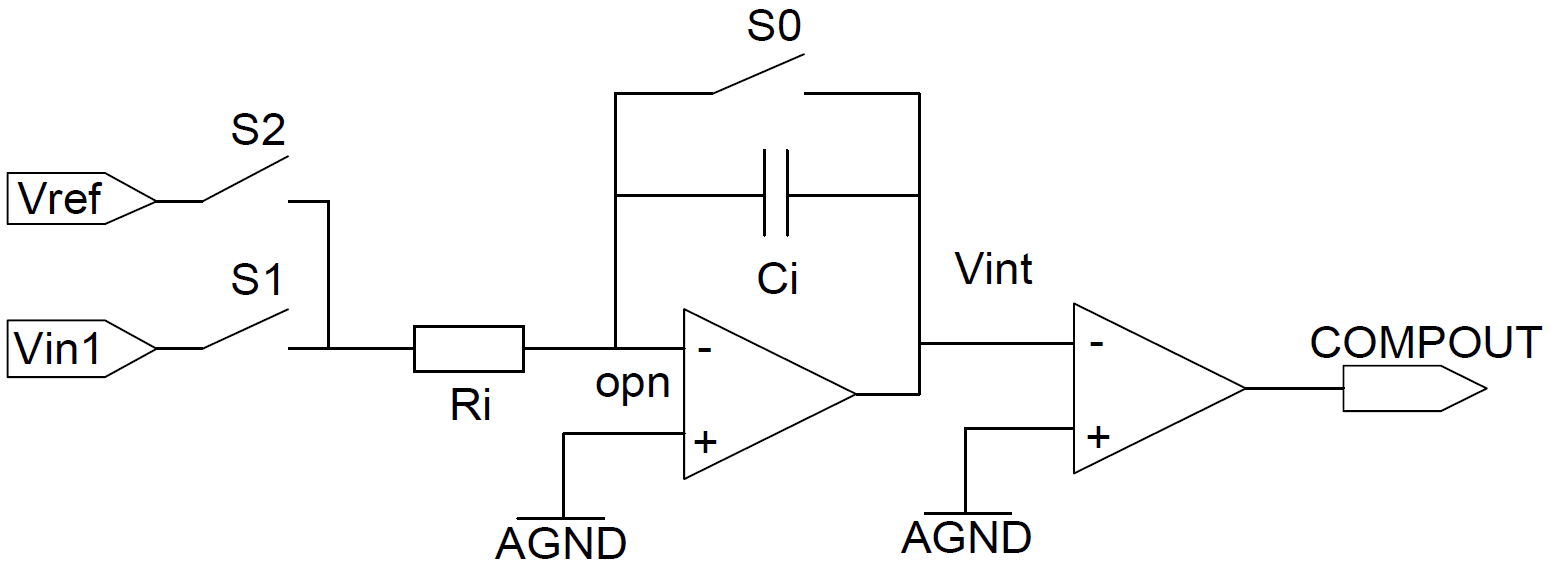
\includegraphics[width=\linewidth]{images/dual_slope_ADC}
\end{minipage}
\begin{minipage}{0.27\linewidth}
    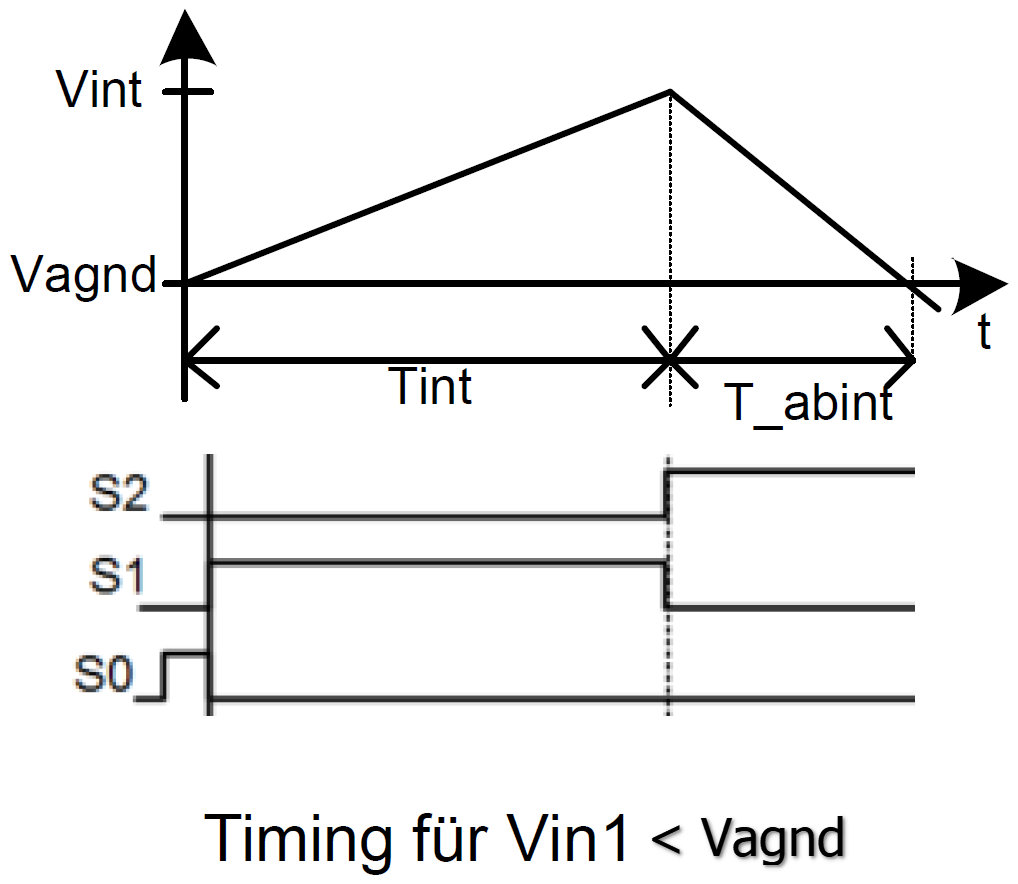
\includegraphics[width=0.83\linewidth]{images//dual_slope_ADC_timing}
\end{minipage}
    \hfill
\begin{minipage}{0.29\linewidth}
    \centering
    $ \boxed{  V_{\rm int} = \frac{\overline{V_{\rm in}} \cdot T_{\rm int}}{R_i \cdot C_i} } $

    $ \boxed{  V_{\rm abint} = \frac{V_{\rm ref} \cdot T_{\rm abint}}{R_i \cdot C_i}  } $ 
\end{minipage}
    
$ \boxed{ \text{DC: } V_{\rm int} = V_{\rm AGND}- \frac{1}{R_i \cdot C_i} \, (V_{\rm in1}- V_{\rm AGND}) \cdot T_{\rm int} } $ 
\quad $\boxed{ \Delta V_{\rm abint} = - \Delta V_{\rm int} }$

$ \boxed{ \Delta V_{\rm abint} = V_{\rm AGND} - V_{\rm int} = - \frac{1}{R_i \cdot C_i} \, (V_{\rm ref} - V_{\rm AGND}) \cdot T_{\rm abint} }$ 
\quad $\boxed{ T_{\rm abint} = - \frac{V_{\rm in1} \cdot T_{\rm int}}{V_{\rm ref}} }$
  
$\boxed{\text{Allgemein: } V_{\rm int} = \int\limits_0^{T_{\rm int}} - \frac{1}{R_i \cdot C_i} \, V_{\rm in1} \, \diff t + V_{\rm int,0} }$
\quad 
$ \boxed{ -\frac{\overline{V_{\rm in}}}{V_{\rm ref}}= \frac{T_{\rm abint}}{T_{\rm int}} = \frac{n \cdot T_{\rm clk}}{N \cdot T_{\rm  clk} } }$


\subsubsection{Frequenzverhalten vom Dual-Slope-Wandler}

Frequenzen $f = \frac{1}{T}$ , wobei $T$ der Intergrationszeit entspricht, werden perfekt unterdrückt \\
$\Rightarrow$ Integrationszeit $T = 20 \, \mathrm{ms}$ unterdrückt Netzbrumm von $50 \, \mathrm{Hz}$


\subsection{Single-Slope-Wandler}

\begin{minipage}[c]{0.52\columnwidth}
    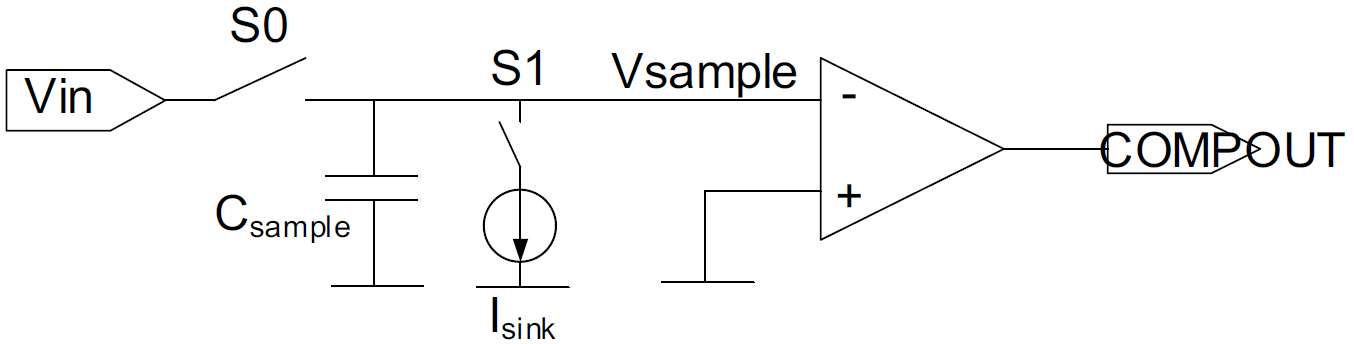
\includegraphics[width=\columnwidth]{images/single-slope-wandler.png}
\end{minipage}
\hfill
\begin{minipage}[c]{0.38\columnwidth}
    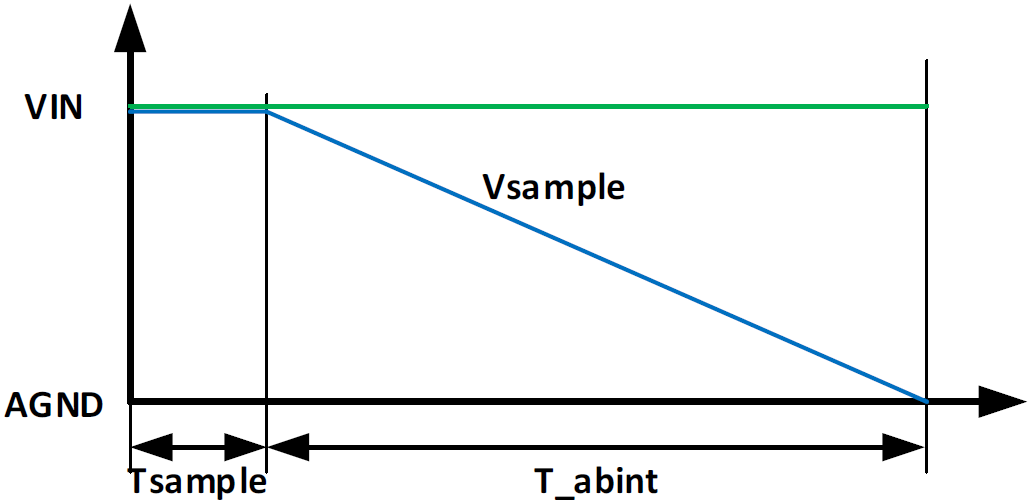
\includegraphics[width=\columnwidth]{images/single-slope-wandler_timing.png}
\end{minipage}

\begin{minipage}[t]{0.48\columnwidth}
    \begin{itemize}
        \item Einfacher als Dual-Slope
        \item $V_ {\rm in}$ wird auf $C_{\rm sample}$ übertragen
        \item $C_{\rm sample}$ wird mit $I_{\rm sink}$ entladen
        \item Zeit bis $V(C_{\rm sample}) = 0$ wird gemessen
    \end{itemize}
\end{minipage}
\hfill
\begin{minipage}[t]{0.48\columnwidth}
    \begin{itemize}
        \item[+] Kein OpAmp, nur zwei Schalter
        \item[+] Schnell, da $T_{\rm sample} < T_{\rm int}$
        \item[-] $V_{\rm in} \sim T_{\rm abint}, \, C_{\rm sample}, \, I_{\rm sink}$
        \item[-] $C_{\rm sample}$ und $I_{\rm sink}$ streuen stark
    \end{itemize}
\end{minipage}


\subsection{Dual-Slope-Wandler für pos. und neg. Eingangsspannungen}

\begin{minipage}[c]{0.52\columnwidth}
    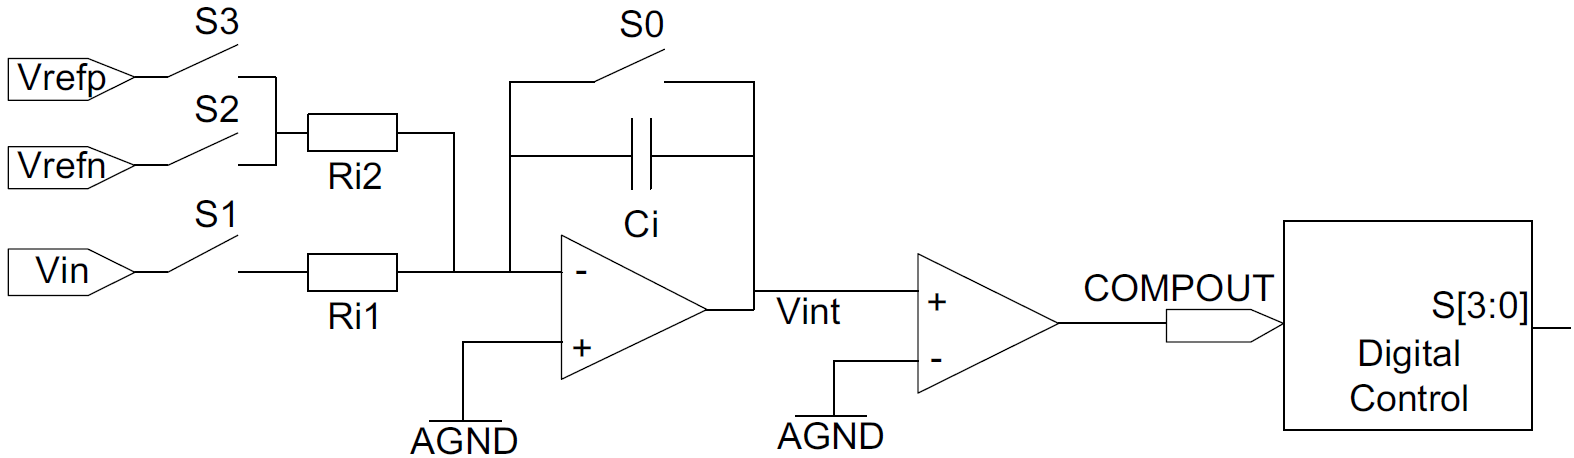
\includegraphics[width=\columnwidth]{images/dual_slope_ADC_pos_neg.png}
\end{minipage}
\hfill
\begin{minipage}[c]{0.37\columnwidth}
    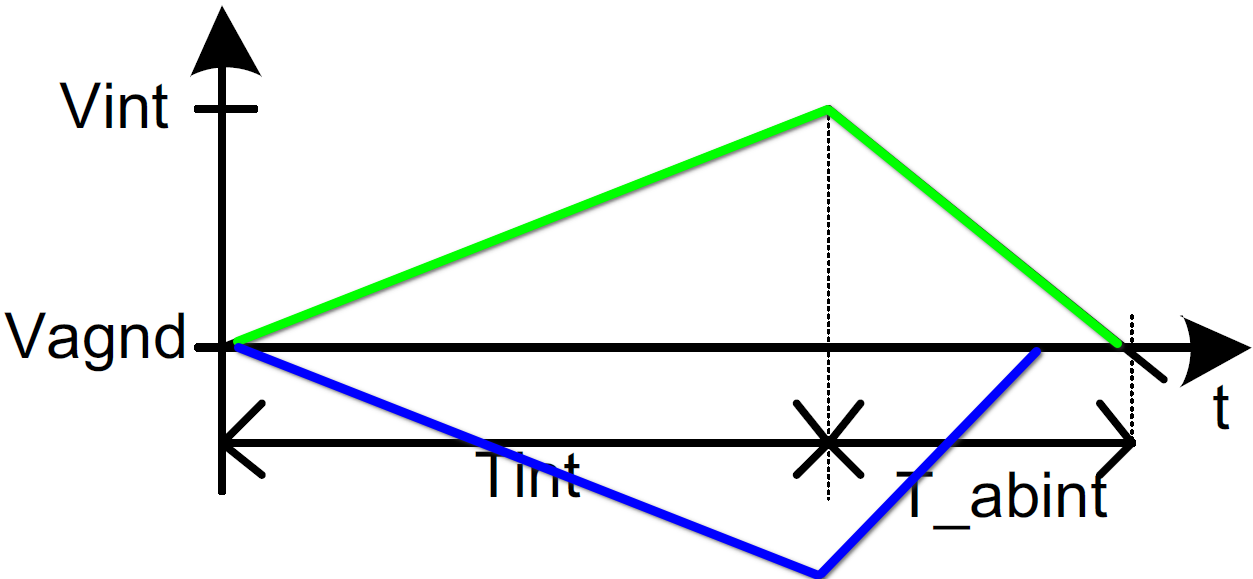
\includegraphics[width=\columnwidth]{images/dual_slope_ADC_pos_neg_timing.png}
\end{minipage}

\begin{minipage}[t]{0.48\columnwidth}
    \begin{itemize}
        \item Auf- und Abintegration wechseln ab
        \item Je nach Komparator-Ausgang wird S2 oder S3 geschlossen
    \end{itemize}
\end{minipage}
\hfill
\begin{minipage}[t]{0.48\columnwidth}
    \begin{itemize}
        \item Für \cgn{$V_{\rm in} < V_{\rm AGND}$} wird in richtung positive Speisung integriert
        \item Für \cbl{$V_{\rm in} > V_{\rm AGND}$} wird in richtung GND integriert
    \end{itemize}
\end{minipage}


\subsubsection{Eigenschaften von Dual-Slope-Wandlern}

\begin{minipage}[t]{0.48\columnwidth}
    \begin{itemize}
        \item Unabhängig von Bauteiltoleranzen
        \item Höhere Auflösung bedingt längere Integrationszeit (bei fixem clk) 
            \textrightarrow\ Doppelte Zeit für 1 zusätzliches Bits
    \end{itemize}
\end{minipage}
\hfill
\begin{minipage}[t]{0.48\columnwidth}
    \begin{itemize}
        \item Höhere Frequenzen werden stärker unterdrückt \textrightarrow\ reduziert Bandbreite
        \item Auflösung wird gegen Bandbreite getauscht
    \end{itemize}
\end{minipage}

